\documentclass[aip,pop,amsmath,amssymb,reprint,superscriptaddress]{revtex4-1} %preprint version
\usepackage{graphicx}% Include figure files
\usepackage{dcolumn}% Align table columns on decimal point
\usepackage{bm}% bold math

    \renewcommand{\topfraction}{0.9}    % max fraction of floats at top
    \renewcommand{\bottomfraction}{0.8}    % max fraction of floats at bottom
    \setcounter{topnumber}{2}
    \setcounter{bottomnumber}{2}
    \setcounter{totalnumber}{4}     % 2 may work better
    \setcounter{dbltopnumber}{2}    % for 2-column pages
    \renewcommand{\dbltopfraction}{0.9}    % fit big float above 2-col. text
    \renewcommand{\textfraction}{0.07}    % allow minimal text w. figs
    \renewcommand{\floatpagefraction}{0.7}    % require fuller float pages
    \renewcommand{\dblfloatpagefraction}{0.7}    % require fuller float pages
    \setlength{\abovecaptionskip}{5pt}
    \setlength{\belowcaptionskip}{5pt}
    \setlength{\parskip}{0pt}
    \setlength{\textfloatsep}{5pt} 

\begin{document}
\title{Obseravation a coherent Drift-Rotational modes with Strong Driven Rotation on the Large Plasma Device}
\author{D.A. Schaffner}
\author{T.A Carter}
\author{G.D. Rossi}
\author{D.S. Guice}
\author{J.E. Maggs}
\author{S. Vincena}
\author{B. Friedman}
\affiliation{Department of Physics and Astronomy, University of California, Los Angeles}
\date{\today}
\begin{abstract}
The instabilities observed on the Large Plasma Device (LAPD) [W. Gekelman, \textit{et. al}, Rev. Sci. Instr. \textbf{62}, 2875 (1991)] are explored in conjunction with a the ability to finely adjust azimuthal flow and flow shear.

\end{abstract}
\maketitle

\section{Introduction}

\section{Observation of Coherent Modes}

Flucutation data from a recently conducted study of finely controlled azimuthal rotation on the LAPD~\cite{schaffner12} shows the emergence of a coherent mode with increasing limiter bias and thus azimuthal flow.

\begin{figure}[!htbp]
\centerline{
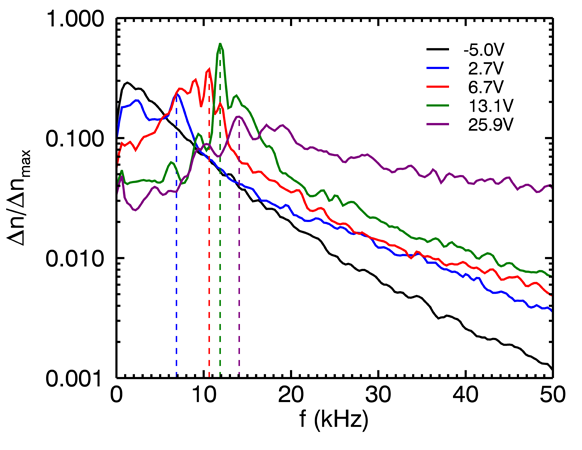
\includegraphics[width=8.5cm]{dens_spec_limedge_zoom.png}}% made using plot_density_spectra_mode_zoom_highbias.pro
\caption{\label{fig:dens_spec_limedge_zoom} Coherent modes for various biases}
\end{figure}

Figure~\ref{fig:dens_spec_limedge_zoom} shows the frequency spectra for various biases for frequencies up to 50kHz and focused in the region right around the limiter edge, where the presense of the coherent mode is strongest. Compared to the minimum flow case (Limiter-Anode = -5.0V), where the fluctuation spectrum is broadband, a clear peaks in the spectra emerge starting at a Limiter-Anode voltage difference of 2.7V and increasing in power and frequency up to a voltage difference of 13.1V. The highest bias listed, with a voltage difference of 25.9V, shows a reduction in power and less distinct peaks.

\section{Conclusions}

The authors would like to thank Zoltan Lucky and Marvin Drandell for their valuable technical support.  This work
was supported by the National Science Foundation (PHY-0903913) and performed using the Basic Plasma Science Facility at UCLA. The BaPSF is funded by the
Department of Energy and NSF.

\providecommand{\noopsort}[1]{}\providecommand{\singleletter}[1]{#1}%
\begin{thebibliography}{10}

%shearing theory
\bibitem{burrell97}
K. Burrell, Phys. Plasmas {\bf 4},  1499  (1997).

\bibitem{burrell99}
K. Burrell, Phys. Plasmas {\bf 6},  4418  (1999).

\bibitem{terry00}
P. Terry, Rev. Mod. Phys. {\bf 72},  109  (2000).

\bibitem{oost03}
G. Van Oost , J. Adamek and V. Antoni, P. Balan, J.A. Boedo, P. Devynck, I. Duran, L. Eliseev, J.P. Gunn, M. Hron, C. Ionita, S. Jachmich, G.S. Kirnev, E. Martines, A. Melnikov, R. Schrittwieser, C. Silva, J. Stockel, M. Tendler, C. Varandas, M. Van Schoor, V. Vershkov and R.R. Weynants, Plas. Phys. Control Fusion {\bf 48}, 621 (2003).

\bibitem{sakai93}
O. Sakai, Y. Yasaka and R. Itatani, Phys. Rev. Lett. {\bf 70},  4071 (1993).

\bibitem{maggs07}
J.E. Maggs, T.A. Carter and R.J. Taylor, Phys. Plasmas {\bf 14},  052507  (2007).

\bibitem{carter09}
T.A. Carter and J.E. Maggs, Phys. Plasmas {\bf 16},  012304  (2009).

\bibitem{schaffner12}
D.A. Schaffner, T.A. Carter, G.D. Rossi, D.S. Guice, J.E. Maggs, S.Vincena and B. Friedman, Phys. Rev. Lett. {\bf 109}, 135002 (2012).

\bibitem{burrell92}
K.H. Burrell, T.N. Carlstrom, E.J. Doyle, D. Finkenthal, P. Gohil, R.J. Groebner, D.L. Hillis, J. Kim, H. Matsumoto, R.A. Moyer, T.H. Osborne, C.L. Rettig, W.A. Peebles, T.L. Rhodes, H. St.John, R.D. Stambaugh, M.R. Wade and J.G. Watkins, Plas. Phys. Control Fusion {\bf 34}, 1859 (1992). 

\bibitem{wagner07}
F. Wagner, Plas. Phys. Control Fusion {\bf 49}, B1 (2007).

\bibitem{taylor89}
R.J. Taylor, M.L. Brown, B.D. Fried, H. Grote, J.R. Liberati, G.J. Morales, P. Pribyl, D. Darrow and M. Ono, Phys. Rev. Lett. {\bf 63},  2365  (1989).

\bibitem{weynants92}
R.R. Weynants, G. Van Oost, G. Bertschinger, J. Boedo, P. Brys, T. Delvigne, K.H. Dippel, F. Durodie, H. Euringer, K.H. Finken, D.S. Gray, J.D. Hey, D.L. Hillis, J.T. Hogan, L. Konan, R. Leners, A.M. Messian, A. Pospieszczyck, U. Samm, R.P. Schorn, B. Schweer, G. Telesca, R. Vannieuwenhove and P.E Vandenplas, Nucl. Fusion {\bf 32},  837  (1992).

\bibitem{weynants98}
R.R. Weynants, S. Jachmich and G. Van Oost, Plas. Phys. Control Fusion {\bf 40}, 635 (1998).

\bibitem{boedo00}
J. Boedo, D. Gray, S. Jachmich, R. Conn, G.P. Terry, G. Tynan, G. Van Oost, R.R. Weynants and TEXTOR Team, Nucl. Fusion {\bf 40},  7  (2000).

\bibitem{boedo02}
J.A. Boedo, D.S. Gray, P.W.Terry, S. Jachmich, G.R. Tynan, R.W. Conn and TEXTOR-94 Team, Nucl. Fusion, {\bf 42}, 117 (2002).

\bibitem{biglari90}
H. Biglari, P.H. Diamond and P.W. Terry, Phys. Fluids B. {\bf 2},  1  (1990).

\bibitem{shaing90}
K.C. Shaing, E.C. Crume and W.A. Houlberg, Phys. Fluids B {\bf 2}, 6 (1990).

\bibitem{zhang92}
Y.Z. Zhang and S.M. Mahajan, Phys. Fluids B {\bf 4}, 1385 (1992).

\bibitem{zhang93}
Y.Z. Zhang and S.M. Mahajan, Phys. Fluids B {\bf 5}, 7 (1993).

\bibitem{ware96}
A.S. Ware, P.W. Terry, P.H. Diamond and B.A. Carreras, Plasma Phys. Control Fusion {\bf 38},  1343  (1996).

\bibitem{ware98}
A.S. Ware, P.W. Terry, B.A. Carreras and P.H. Diamond, Phys. Plasmas {\bf 5}, 173 (1998).

\bibitem{terry01}
P.W. Terry, D.E. Newman and A.S. Ware, Phys. Rev. Lett. {\bf 87}, 185001  (2001).

\bibitem{kim03}
E.-J. Kim and P.H. Diamond, Phys. Rev. Lett. {\bf 90}, 7 (2003).

\bibitem{kim04}
E.-J. Kim, P.H. Diamond and T.S. Hahm, Phys. Plasmas {\bf 11},  10  (2004).

\bibitem{newton11}
A.P.L. Newton and E.-J. Kim, Phys. Plasmas {\bf 18}, 052305 (2011).

\bibitem{gek91}
W. Gekelman, H. Pfister, Z. Lucky, J. Bamber, D. Leneman and J. Maggs, Rev. Sci. Instrum. {\bf 62},  2875  (1991).

\bibitem{hahm94}
T.S. Hahm, Phys. Plasmas {\bf 1}, 2940 (1994).

\bibitem{leconte06}
M. Leconte, P. Beyer, S. Benkadda and X.Garbet, Phys. Plasmas {\bf 13} 112301 (2006).

\bibitem{newton07}
A.P.L. Newton and E.-J. Kim, Phys. Plasmas {\bf 14}, 122306 (2007).

\bibitem{terry06}
P.W. Terry and R. Gatto, Phys. Plasmas {\bf 13}, 062309 (2006).

\bibitem{staebler13}
G.M. Staebler, R.E. Waltz, J. Candy and J.E. Kinsey, Phys. Rev. Lett. {\bf 110}, 055003, (2013)).

\bibitem{friedman12}
B. Friedman, T.A. Carter, M.V. Umansky, D. Schaffner and B. Dudson, Phys. Plasmas {\bf 19}, 102307 (2012).

\bibitem{umansky11}
M. Umansky {\it et~al.}, Phys. Plasmas {\bf 18},  055709  (2011).

\bibitem{popovich10BOUT}
P.Popovich, M.V. Umansky, T.A. Carter and B. Friedman, Phys. Plasmas {\bf 17}, 122312 (2010).

\end{thebibliography}
\end{document}
